\title{Synthesizing Static Analyses from Examples}
\author{
        Martin Kellogg \\
        University of Washington
            \and
        Everett Maus\\
        Microsoft Corporation
}


\documentclass[10pt,conference]{IEEEtran}

\usepackage{graphicx}

\begin{document}

\maketitle

\begin{abstract}

Constructing static analyses requires a great deal of
manual, expert programmer effort. We propose a framework
for automatically synthesizing the implementation of analyses
from examples of the analysis in action, which will greatly
reduce the effort required to build and deploy static analysis
tools.

\end{abstract}

\section{Motivation}

A well-designed static analysis (or, equivalently, a type system or abstract interpretation)
can allow developers to find bugs in their code quickly and with little manual effort,
or even avoid entire classes of errors by verifying that their code can never
do some undesirable thing. However, these benefits come at a
cost---developing such a static analyses 
requires an expert to spend a long time
both designing and implementing the static analysis (for instance, one
interesting static analysis that checks the types of the arguments to a format string was sufficient
to publish a paper at a recent top-tier software engineering venue~\cite{format-string-checker}.
Worse, the cost to build such static analyses means that many that are
designed by the research community are never engineered to the level of practicality and precision
that would be required to run on real-world code, so programmers
never gain their benefits.

We propose to deploy state-of-the-art techniques from the domain of program
synthesis to allow programmers to specify a static analysis by providing
examples of the code that the analysis should and should not permit.
This will relieve the burden of actually building the infrastructure
required to deploy complex static analyses, so that specialized analyses
with the precision required of industrial-strength tools can be built without
needing an intimate knowledge of the theory of abstract interpretation,
which will allow non-specialists (like industrial programmers) to become
static analysis builders.

\section{Background}

\subsection{Abstract Interpretation}

\begin{figure}
 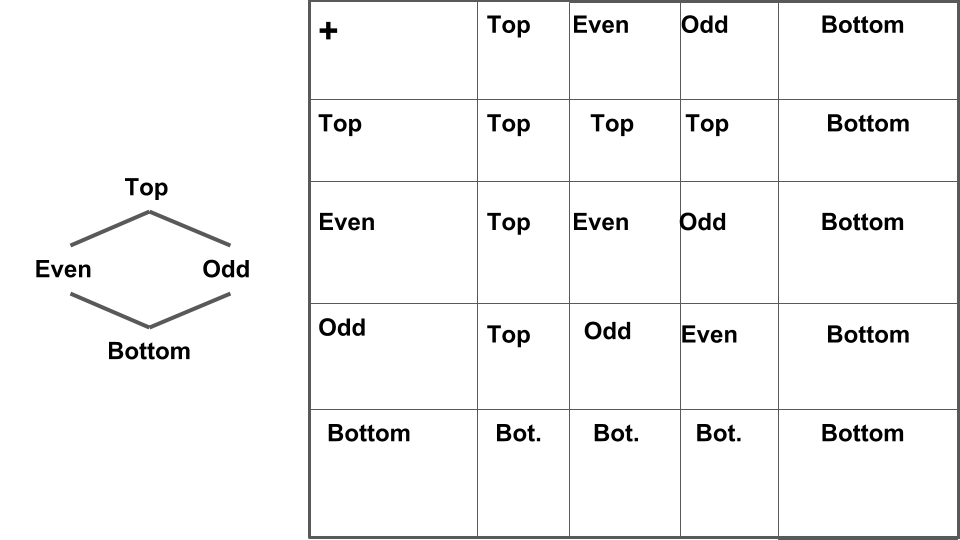
\includegraphics[width=\linewidth]{parity.png}
 \caption{A lattice of abstract domains and a transfer function
   for plus, for an abstract analysis that tracks the parity of
 a value.}
\label{fig-parity}
\end{figure} 

A static analysis can be formally modelled
as a lattice of \textit{abstract domains} and a set of \textit{transfer functions}
that transform abstract domains to other abstract domains when some
program operator is encountered~\cite{cousot77}. The analysis then proceeds by symbolically
interpreting the program being analyzed, replacing each concrete value with
an abstract domain determined by applying the transfer functions. An example
lattice and transfer function for the plus operator are given in Figure~1.
The analysis shown in Figure~1 is a parity analysis---it keeps track of
whether integers are even or odd. There are also two other possiblities:
the integer could be either even or odd (the ``top'' type) or it could
be \textit{both} even and odd---such as in dead code (represented by the
``bottom'' type). The lattice shows how these abstract domains are related,
with a subtyping relationship represented by the lines---any abstract domain
with a line going to another abstract domain higher in the lattice is a strict
subset of the higher abstract domain (so, for instance, top contains both
all even integers and all odd integers, so both even and odd are its subtypes).
/iffalse
  (Comment that doesn't affect the doc yet)
  My opinion is that we aren't really modelling subtyping in the traditional meaning
  of the term in Computer Science with the latice--it's not an "is-a" relationship 
  (i.e. claiming 'Bottom is-a Even' doesn't line up with an intuitive grasp of the model).
  Subsets seem to more accurately model the behavior of the lattice--this would
  mean changing 'both' to 'neither' and rephrasing the preceeding sentence.
/fi
The transfer function shows how the result of the plus operation is related
to its operands. We represent this as a matrix, with the top row and leftmost
column representing the abstract domains of the operands, and the interior
parts of the matrix representing the abstract domain of the result. So,
as an example, if $a$ is odd and $b$ is bottom, then $a + b$ is bottom,
because the entry for odd and bottom in the matrix is bottom.

\subsection{Synthesis}

The field of program synthesis uses SMT solvers to
automatically build programs based on a set of constraints provided
by the programmer. Modern SMT solvers, such as z3~\cite{z3}, are able
to solve equations involving millions of variables extremely quickly, despite 
the problem they solve (boolean satisfiabilty) being known to be NP-complete~\cite{cook71complexity}. 
These modern solvers allow the synthesis of, for example, memory models for modern architectures
in a few seconds from the architecture's litmus tests~\cite{bornholt17}.
Synthesis works by reducing the constraints provided by the user
(litmus tests, a formal specification, etc.) to a boolean satisfiability
problem, calling the solver, and then translating the result back into
a program. Because the search space for programs is so large, practical
synthesis techniques use \textit{sketches} of the solution to reduce
the search space. A sketch is an outline of the form of the answer,
such as a program with some expressions missing.

\section{Technical Approach}

\begin{figure}
 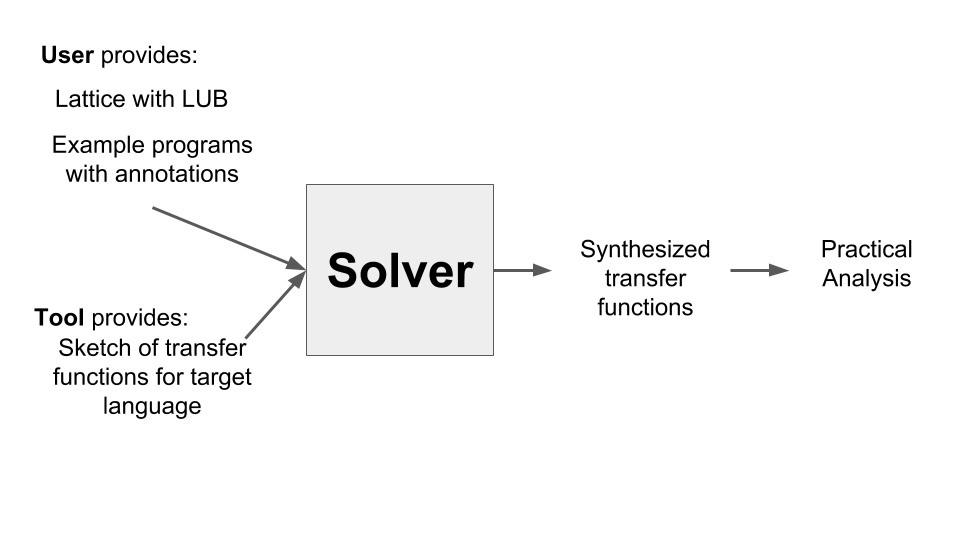
\includegraphics[width=\linewidth]{arch.png}
 \caption{The proposed architecture for the tool.
   Examples are translated to contraints and a sketch of the transfer function is built.
   These are passed to a solver, and then the resulting transfer function is translated into
 a practical analysis.}
\label{fig-arch}
\end{figure} 

Our proposed approach involves three steps.
First, translate examples of the static analysis on sample programs
into constraints on the transfer function and create
a sketch of the transfer functions for the target language.
Second, pass those constraints and the sketch to the solver;
the result of that solver call is a filled-in transfer
function. Finally, translate the produced transfer function
into an actual analysis that can be run by a programmer.
A diagram of this architecture is shown in Figure~2.

The lattice for the abstract analysis is provided by
the programmer, since it must be known to write the examples.
The examples would take the form of code annotated with the
abstract domains (in the same way typed languages have type annotations).
The produced transfer function, along with the known lattice,
should give enough information to mechanically create the practical
analysis on top of a framework like the Checker Framework~\cite{checker-framework}.

\section{Implementation and Evaluation}

We propose to target the IMP programming language~\footnote{https://www.seas.upenn.edu/~cis500/current/sf/Imp.html}
during this course project, with the idea that we would be able to re-use the internals
(i.e. the code that calls the solver) if the project is successful in
a version of the tool that targetted a more practical language like Java.
We will use z3~\cite{z3} as our solver, and transform the IMP programs directly
into SMT2 constraints using a modified IMP interpreter to symbolically evaluate
the examples. Because of the (time) constraints of a course project, we will not
implement the last stage of our proposed approach, but rather stop with a
synthesized transfer function.

We will evaluate our approach by comparing the synthesized transfer
functions for several analyses to the ground truth accepted transfer
functions. The analyses we will consider are: a parity analysis,
a signedness analysis, a null-pointer analysis (using a version of
IMP augmented with a heap), and a range analysis, in that order.
Evaluation metrics will include whether we are able to reproduce
the correct transfer functions, and how many example test cases
are required in each case.

\section{Future Work}

A conference-length paper on this topic would extend the tool to operate
on Java programs, with the final goal being the replication of
existing Checker Framework checkers using only those checkers'
test suites. This would require building signficantly more
complex transfer functions---and probably would require
a meta-sketching approach~\cite{metasketching} that tried several levels of
sketches for the transfer functions (moving from
refining only the result of the expression to
refining multiple variables to a flow-sensitive refinement, etc.).
This would also require implementing the last stage of the tool, which
translates the synthesized transfer function into a Checker Framework
checker.

\section{References}

\begingroup
\renewcommand{\section}[2]{}%

% The following two commands are all you need in the initial runs of
% your .tex file to produce the bibliography for the citations in your
% paper.
\bibliographystyle{plain}
\bibliography{genprog-bib/merged}
% You must have a proper ``.bib'' file
% and remember to run:
% latex bibtex latex latex
% to resolve all references
%
% ACM needs 'a single self-contained file'!
%
\endgroup

\end{document}
This is never printed
